%%%%%%%%%%%%%%%%%%%%%%%%%%%%%%%%%%%%%%%%%%%%%%%%%%%%%%%%%%%%%%%%%%%%%%%%%%%%
%% Author template for Management Science (mnsc) for articles with no e-companion (EC)
%% Mirko Janc, Ph.D., INFORMS, mirko.janc@informs.org
%% ver. 0.95, December 2010
%%%%%%%%%%%%%%%%%%%%%%%%%%%%%%%%%%%%%%%%%%%%%%%%%%%%%%%%%%%%%%%%%%%%%%%%%%%%
\documentclass[mnsc]{informs3}
%\documentclass[mnsc,blindrev]{informs3}
%\documentclass[mnsc,nonblindrev]{informs3} % current default for manuscript submission

\OneAndAHalfSpacedXI
%%\OneAndAHalfSpacedXII % Current default line spacing
%%\DoubleSpacedXII
%%\DoubleSpacedXI

% If hyperref is used, dvi-to-ps driver of choice must be declared as
%   an additional option to the \documentclass. For example
%\documentclass[dvips,mnsc]{informs3}      % if dvips is used
%\documentclass[dvipsone,mnsc]{informs3}   % if dvipsone is used, etc.

% Private macros here (check that there is no clash with the style)
%%%%%%%% Linkage
\usepackage{xurl}
\usepackage{hyperref}
\hypersetup{colorlinks=true,citecolor=blue,urlcolor=blue}

%%%%%%%% Colored underline
\usepackage{ulem}
\usepackage{soul}
\makeatletter
    \newcommand{\coloruline}[2]{%
        \newcommand\temp@reduline{\bgroup\markoverwith
            {\textcolor{#1}{\rule[-0.5ex]{2pt}{0.4pt}}}\ULon}%
        \temp@reduline{#2}%
    }
    \newcommand{\coloruwave}[2]{%
        \UL@protected\def\temp@uwave{\leavevmode \bgroup 
        \ifdim \ULdepth=\maxdimen \ULdepth 3.5\p@
        \else \advance\ULdepth2\p@ 
        \fi \markoverwith{\textcolor{#1}{\lower\ULdepth\hbox{\sixly \char58}}}\ULon}
        \font\sixly=lasy6 % does not re-load if already loaded, so no memory drain.
        \temp@uwave{#2}%
    }
\makeatother

%%%%%%%% Algorithm
\usepackage{algorithm}
\usepackage{algorithmic}

%%%%%%%% Table, Figure and Diagram
%%%%%%%%%% Table
\usepackage{makecell}
\usepackage{tabularx}
\usepackage{array}
\usepackage{booktabs}
\usepackage{multirow}
%%%%%%%%%% Figure
\usepackage{float}
\usepackage{graphicx}
\usepackage{graphics}
\usepackage{caption,}
\usepackage{subcaption}
%%%%%%%%%% Diagram Figure
\usepackage{tikz}
\usepackage{varwidth}
%%%%%%%%%% Comments
\usepackage{comment}


% Natbib setup for author-year style
\usepackage{natbib}
 \bibpunct[, ]{(}{)}{,}{a}{}{,}%
 \def\bibfont{\small}%
 \def\bibsep{\smallskipamount}%
 \def\bibhang{24pt}%
 \def\newblock{\ }%
 \def\BIBand{and}%

%% Setup of theorem styles. Outcomment only one.
%% Preferred default is the first option.
\TheoremsNumberedThrough     % Preferred (Theorem 1, Lemma 1, Theorem 2)
%\TheoremsNumberedByChapter  % (Theorem 1.1, Lema 1.1, Theorem 1.2)
\ECRepeatTheorems

%% Setup of the equation numbering system. Outcomment only one.
%% Preferred default is the first option.
\EquationsNumberedThrough    % Default: (1), (2), ...
%\EquationsNumberedBySection % (1.1), (1.2), ...

% For new submissions, leave this number blank.
% For revisions, input the manuscript number assigned by the on-line
% system along with a suffix ".Rx" where x is the revision number.
\MANUSCRIPTNO{MS-0001-1922.65}


%%%%%%%%%%%%%%%%
\begin{document}
%%%%%%%%%%%%%%%%

% Outcomment only when entries are known. Otherwise leave as is and
%   default values will be used.
%\setcounter{page}{1}
%\VOLUME{00}%
%\NO{0}%
%\MONTH{Xxxxx}% (month or a similar seasonal id)
%\YEAR{0000}% e.g., 2005
%\FIRSTPAGE{000}%
%\LASTPAGE{000}%
%\SHORTYEAR{00}% shortened year (two-digit)
%\ISSUE{0000} %
%\LONGFIRSTPAGE{0001} %
%\DOI{10.1287/xxxx.0000.0000}%

% Author's names for the running heads
% Sample depending on the number of authors;
% \RUNAUTHOR{Jones}
% \RUNAUTHOR{Jones and Wilson}
% \RUNAUTHOR{Jones, Miller, and Wilson}
% \RUNAUTHOR{Jones et al.} % for four or more authors
% Enter authors following the given pattern:
%\RUNAUTHOR{}

% Title or shortened title suitable for running heads. Sample:
% \RUNTITLE{Bundling Information Goods of Decreasing Value}
% Enter the (shortened) title:
\RUNTITLE{Information Disclosure in Dynamic Innovation Contests}

% Full title. Sample:
% \TITLE{Bundling Information Goods of Decreasing Value}
% Enter the full title:
\TITLE{Information Disclosure in Dynamic Innovation Contests}

% Block of authors and their affiliations starts here:
% NOTE: Authors with same affiliation, if the order of authors allows,
%   should be entered in ONE field, separated by a comma.
%   \EMAIL field can be repeated if more than one author
\ARTICLEAUTHORS{%
\AUTHOR{Jussi Keppo}
\AFF{NUS Business School and Institute of Operations Research and Analytics\\
	National University of Singapore, Singapore\\
	\EMAIL{keppo@nus.edu.sg}} %, \URL{}}
\AUTHOR{Linsheng Zhuang}
\AFF{Institute of Operations Research and Analytics\\
	National University of Singapore, Singapore\\
	\EMAIL{linsheng.z@u.nus.edu}}
% Enter all authors
} % end of the block

\ABSTRACT{%
...
% Enter your abstract
}%

% Sample
%\KEYWORDS{deterministic inventory theory; infinite linear programming duality;
%  existence of optimal policies; semi-Markov decision process; cyclic schedule}

% Fill in data. If unknown, outcomment the field
\KEYWORDS{Digital Economy, Data Protection Regulation, Innovation Contest} 
%\HISTORY{......}

\maketitle
%%%%%%%%%%%%%%%%%%%%%%%%%%%%%%%%%%%%%%%%%%%%%%%%%%%%%%%%%%%%%%%%%%%%%%

% Samples of sectioning (and labeling) in MNSC
% NOTE: (1) \section and \subsection do NOT end with a period
%       (2) \subsubsection and lower need end punctuation
%       (3) capitalization is as shown (title style).
%
%\section{Introduction.}\label{intro} %%1.
%\subsection{Duality and the Classical EOQ Problem.}\label{class-EOQ} %% 1.1.
%\subsection{Outline.}\label{outline1} %% 1.2.
%\subsubsection{Cyclic Schedules for the General Deterministic SMDP.}
%  \label{cyclic-schedules} %% 1.2.1
%\section{Problem Description.}\label{problemdescription} %% 2.

% Text of your paper here


\section{Introduction}

\begin{itemize}
\item Kaggle\footnote{\url{https://www.kaggle.com}} ...
\item Meta-kaggle dataset \cite{megan_risdal_timo_bozsolik_2022}. 
\end{itemize}

\subsection{Literature Review}

This paper focuses on the two players innovation contest with a continuous time  where the players’ relative position is public information throughout the game.
This is closely related to tug-or-war contest, which, to our knowledge, was first formally given by \citet{Harris1987Race} as a one-dimensional simplification of the multi-stage R\&D race. 
The output processes are model by Brownian motions drifted with effort inputs, which is followed by \cite{budd1993model} who model the state of a dynamic competition of two innovative duopoly firms by a Brownian motion drifted by the effort gap, and solve the equilibrium approximately. 
Furthermore, \citet{Moscarini2011Contest} model the tug-of-war state as the gap of the two outputs directly, and draw an analytical equilibrium of the pure strategies. 

...

Information disclosure in contest - \cite{Bimpikis2019Contest}. 

...

Closest paper - \cite{ryvkin2022fight}.

...




\section{The Model}

% Effort, Output and Gap
Two players, $i$ and $j$, compete for a prize $\theta>0$ in a contest. 
Winner gets the prize and loser gets nothing. 
The contest starts at time zero. 
At every time $t\ge0$, the representative player $i$ chooses an effort level $q_{i,t}$ and burdens a quadratic cost $C_i(q_{i,t}) = c_i q_{i,t}^2/2$, with a lower $c_i$ corresponding to higher ability. 
Denoted by $y_t$ the \textit{output gap} of player $i$ and $j$ at time $t$, driven by
\begin{equation}\label{eq-state-dynamics}
	dy_t = (q_{i,t}-q_{j,t})dt + \sigma dW_t
\end{equation}
where $W_t$ is a Brownian motion and $\sigma>0$ measures the innovation risk.

The contest is equipped with a submission system that allows participants to upload their algorithms at any time and receive immediate feedback. 
For simplicity, we further assume that agents submit their intermediate results whenever they make progress. 
This setup enables the contest organizers to monitor all players’ progress $x_{i,t}$ and $x_{j,t}$ in real time. 
Moreover, the true output level, evaluated by the system, is only known by the game designer but not the two players. 
% Signal
At any time $t>0$, the contest designer emits a \textit{public} signal of the real output gap $y_t$. 
The signal is ambiguous and the game holder controls the ambiguity. 
The dynamic of signal is  
\begin{equation}\label{signal}
	dZ_{t} = y_{t}dt + \frac{dB_{t}}{\sqrt{\lambda}} 
\end{equation}
where $B_{t}$ is standard Brownian motion independent with $(W_{i,t})$ and $(W_{j,t})$, and the parameter $\lambda$ is set by the game holder to control the precision of signal. 
The larger the $\lambda$, the more accurate the signal would be. 

% Bayesian Player
The information set of both players at time $t \ge 0$ is  $I_{t} \equiv \{Z_{s} : 0\le s \le t\}$. 
Player $i$ estimates the unknown output gap $y_t$ based on the information set $I_t$. 
Let $\tilde{y}_t \equiv E(y_{t}|I_t)$ be the estimated output gap and $S_t \equiv E[(\tilde{y}_{t}-y_{t})^2|I_t]$ be the estimation variance. 
According to Chapter 1.2 of \citet{Bensoussan1992Control}, \textit{Kalman-Bucy filter} gives the dynamics of $\tilde{y}_{t}$ and $S_{t}$, 
\begin{align}
	d\tilde{y}_{t} &= (q_{i,t}-q_{j,t})dt + \lambda S_{t}(dZ_{t}-\tilde{y}_{t}dt) 
	\label{filtered-x}\\
	\frac{dS_{t}}{dt} &= \sigma^2 - \lambda S_{t}^2
	\label{filtered-S}
\end{align} 
Hence, the conditional distribution $y_{t}|I_t\sim\mathcal{N}(\tilde{y}_{t},S_{t}|I_t)$ is fully captured by the mean $\tilde{y}_{t}$ and variance $S_{t}$. 
If $\lambda = 0$, we have $S_t = S_0+\sigma^2t$, i.e., the estimation variance is increasing in time linearly. 
If $\lambda > 0$, the solution of (\ref{filtered-S}) is
\begin{equation}\label{S-evolution} 
	S_t = 
	\begin{cases}
        \bar{S} \cdot \tanh\left\{t\cdot\sigma\sqrt{\lambda} +  \tanh^{-1}\left(S_0\big/\bar{S}\right)\right\} & \text{if } S_0 < \bar{S} \\
        \bar{S} & \text{if } S_0 = \bar{S} \\
        \bar{S} \cdot \coth\left\{t\cdot\sigma\sqrt{\lambda} +  \coth^{-1}\left(S_0\big/\bar{S}\right)\right\} & \text{if } S_0 > \bar{S} 
	\end{cases}
\end{equation}
Specifically, $\bar{S} = \sigma / \sqrt{\lambda}$ when $\lambda>0$ and $\bar{S} = \infty$ when $\lambda = 0$. 
Please refer to Appendix~\ref{app-S-equ} for the derivations. 
Figure~\ref{fig-S-evol} shows the evolution of $S_t$ in time: estimation variance $S_t$ converges to \textit{steady state} $\bar{S}$ as time goes by regardless of the starting estimation variance. 
For simplicity, we henceforth assume that $S_0 = \bar{S}$, hence $S_t\equiv \bar{S}$. 

\begin{figure}[!ht]
	\centering
	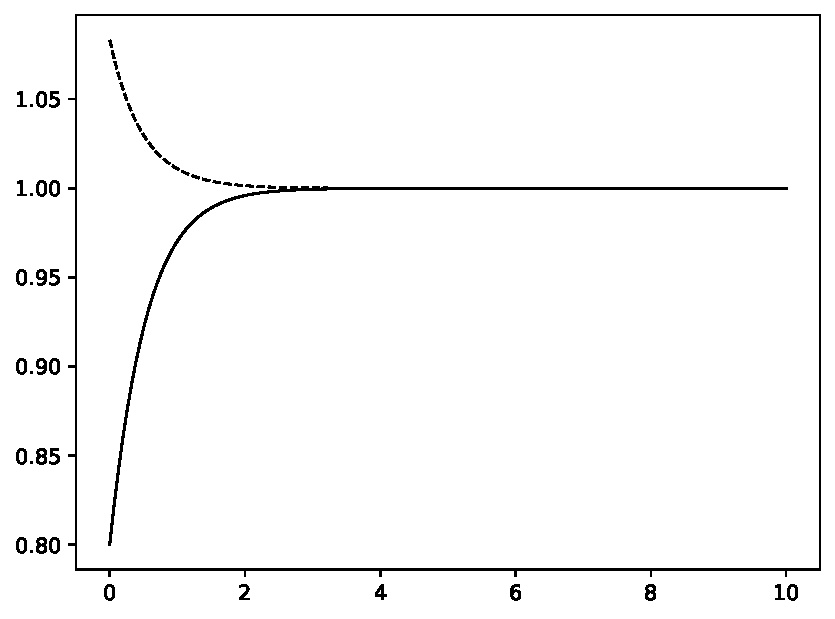
\includegraphics[scale=0.6]{figure_S_evolve.pdf}
	\caption{The evolution of $S_t$ in time $t$, given that $\lambda = 1$ and $\sigma = 1$.} \label{fig-S-evol}
\end{figure}



% Contest Deadline
Following \cite{ryvkin2022fight}, let's consider a dynamic contest with a fixed deadline. 
Suppose the contest is terminated when time $t=T>0$. 
Since the steady state estimation variance $\bar{S}$ is fixed as displayed above, the state of the game is fully characterized by a tuple $(\tilde{y}_t, t)$. 
At any time $0\le t<T$, player $i$ optimizes her effort level $q_{i,\tau}$ in the remaining contest period $\tau\in[t, T)$ according to the following optimization problem, 
\begin{equation}\label{v-def}
	V^i(\tilde{y}_{t}, t ; q_{j,t},\Theta_i) = \max_{\{q_{i,\tau}\}^T_{\tau=t}} 
	\mathbb{E}\left( \theta\cdot1_{\tilde{y}_T>0} - \int^T_tC_i(q_{i,\tau})d\tau \bigg|I_t\right) 
\end{equation}
where $\Theta_i \equiv\{\theta, \lambda, \sigma, c_i\}$, subject to constraints (\ref{filtered-x}), (\ref{filtered-S}) and $q_{i,\tau}\ge0$ for all $\tau\in[t,T)$.
The optimization problem for player $j$ is just symmetric to that of player $i$ as $V^j(\tilde{y}_t, t) = V^i(-\tilde{y}_t, t)$. 
The corresponding Hamilton-Jacobi-Bellman (HJB) equation for player $i$ is 
\begin{equation*}
0 = \max_{q_{i,t}\ge0}\left[-\frac{c_iq_i^2}{2} + V^i_{y}\cdot\left(q_{i,t}-q_{j,t}\right)+V^i_t + \frac{V^i_{yy}}{2}\lambda \bar{S}^2\right]
\end{equation*}
By definition, we have $\lambda \bar{S}^2 = \sigma^2$. 
Under the assumption of inner solution, we plug into the first order conditions $q_{i,t} = V^i_y/c_i$ and $q_{j,t} = -V^j_y/c_j$, we have the system of equations
\begin{equation*}
\begin{aligned}
\frac{1}{2c_i}(V^i_y)^2 + \frac{1}{c_j}V^i_yV^j_y + V^i_t + V^i_{yy}\frac{\sigma^2}{2} = 0\\
\frac{1}{2c_j}(V^j_y)^2 + \frac{1}{c_i}V^j_yV^i_y + V^j_t + V^j_{yy}\frac{\sigma^2}{2} = 0
\end{aligned}
\end{equation*}
subject to boundary conditions $V^i(-\infty, t) = 0$, $V^i(+\infty, t) = \theta$, $V^j(-\infty, t) = \theta$, $V^j(+\infty, t)=0$, $V^i(\tilde{y}_T, T) = \theta \cdot 1_{\tilde{y}_T > 0}$ and $V^j(\tilde{y}_T, T) = \theta \cdot 1_{\tilde{y}_T < 0}$. 


The Nash equilibrium is summarized in the following lemma. 
We include a simplified version of the proof in the appendix: 

\begin{lemma}[\citealt{ryvkin2022fight}]
In the Markov perfect equilibrium, the players’ efforts in state $m_{i(j)}(\tilde{y}_t, t) :\mathbb{R}\times[0, T)\to\mathbb{R}_+$ are given by
\begin{equation}\label{eq-equilibrium-effort}
m_{i(j)}(\tilde{y}_t, t) = \frac{e^{-z^2/2}}{\sqrt{2\pi\sigma^2(T-t)}}\cdot \frac{\sigma^2}{2}\left[\gamma(\rho_{i}) + \gamma(\rho_{j})\right]\left[1-\rho(z)^2\right]\left[1 \pm \rho(z)\right]
\end{equation}
where $z = \tilde{y}_t / (\sigma\sqrt{T-t})$, $\rho(z) = \gamma^{-1}\left(\Phi(z)\left[\gamma(\rho_{i})+\gamma(\rho_{j})\right]-\gamma(\rho_{j})\right)$ and 
\begin{equation*}
\gamma(u) = \frac{u}{1-u^2} + \frac{1}{2}\ln\frac{1+u}{1-u},\quad u\in(-1,1)
\end{equation*}
\begin{equation*}
\rho_{i} = \frac{e^{w_{i}}+e^{-w_{j}}-2}{e^{w_{i}}-e^{-w_{j}}},
\quad
\rho_{j} = \frac{e^{w_{j}}+e^{-w_{i}}-2}{e^{w_{j}}-e^{-w_{i}}},
\quad
w_{i(j)} = \frac{\theta}{\sigma^2 c_{i(j)}}.
\end{equation*}
\end{lemma}

The variables $w_{i(j)}$ represent the abilities of two players, while $\rho_{i(j)}$ normalizes $w_{i(j)}$ into the interval $(-1, 1)$. 
It is not hard to see that $\gamma(\cdot)$ is strictly increasing on $(-1,1)$, ranging from $-\infty$ to $+\infty$. 
Moreover, the equilibrium effort $m_{i(j)}$ can be represented to the product of $\phi(y; 0, \sigma^2(T-t))$, the probability density of normal distribution with mean zero and variance $\sigma^2(T-t)$ at the state $y$ and an amplitude factor that only depends on the composite variable $z$. 








\section{Estimation}

In this section, we describe the estimation procedure. 
We first outline the data generation process, establishing the connection between the empirical data and the theoretical model discussed previously.
Then, we introduce a structural estimation method using Bayesian framework.

\subsection{Data Generating Process}

For each contest on Kaggle, the observable information can be classified into three primary components: 

%% Data: Contest setting
The first component consists of essential contest details, including the contest duration, prize structure, information disclosure policy, and other governing rules.
Contrary to the assumptions of our model, a typical contest usually involves multiple teams rather than just two.
We index the participating teams of the contest by $i\in\{1, 2, ..., n\}$. 
To fully leverage the potential of the data and establish a connection with our theoretical model, let's assume that each participant perceives a competitor they are playing against at every moment, denoted as $j$. 
This perceived competitor is typically understood as the most prominent individual on the leaderboard, i.e., the person ranked first.
When team $i$ themselves hold the top position, their perceived competitor is the individual who poses the greatest threat, namely the person ranked second.
Furthermore, the contests may feature intricate prize structures, such as the provision of multiple awards, rather than adhering to a winner-takes-all format.
The issue will be discussed in Section~\ref{sec-kaggle-application}. 

%% Data: Submissions
The second component captures the submission events of each player $i$ to the system, denoted by the sequence $\{\hat{t}^i_k\}_{k=1}^{N_i}$.
Here, $N_i$ represents for the total number of submissions by player $i$, and $t$ represents for the time of each submission. 
We understand the submission events of player $i$ and $j$ as two conditional independent inhomogeneous Poisson processes, driven by the intensity functions $\tau_i(t)$ and $\tau_j(t)$.\footnote{That is, given the intensity functions $\tau_i(t)$ and $\tau_j(t)$, the submission events $\{\hat{t}^i_k\}_{k=1}^{N_i}$ and $\{\hat{t}^j_k\}_{k=1}^{N_i}$ are mutually independent.}
Then, during any time interval $\mathcal{S}$ of the contest duration $\mathcal{T}$, the Poisson arrival rate of submissions of the representative player $i$ is given by $\int_{s\in\mathcal{S}}\tau_i(s)ds$. 
We assume the submission intensity $\tau_i(t)$ is proportional to the effort level $m_i(\tilde{y}_t, t)$. More specifically, 
\begin{equation}\label{eq-model-intensity}
\tau_i(t) = r \cdot m_i(\tilde{y}_t, t)
\end{equation}
where $r>0$ is the common ratio of submission intensity and effort. 

%% Data: Leaderboard
The third component of the observed data is an open leaderboard that records the real-time rankings and scores of each participant, denoted by $\hat{x}^i_t$. 
We interpret the difference in scores between $i$ and $j$ displayed on the leaderboard as the signal $Z_t$ (defined in (\ref{signal})) released by the contest organizer. 
Specifically, let's denote $\hat{y}_t = \hat{x}^i_t - \hat{x}^j_t$ the gap between displayed scores, and interpret it as the signal intentionally released by the contest organizer: 
\begin{equation}\label{eq-model-signal}
dZ_t = \hat{y}_tdt
\end{equation}
As indicated in (\ref{signal}), we assume that $\hat{y}_t$ represents a noisy signal, with its precision governed by $\lambda$.
Moreover, according to (\ref{eq-state-dynamics}), the observed real-time gap $\hat{y}_t$ on leaderboard evolves as 
\begin{equation}\label{eq-leaderboard-gap}
d\hat{y}_t = \left[m_i(\tilde{y}_t, t) - m_j(\tilde{y}_t, t)\right]dt + \sigma dW_{t} + \frac{dB_t}{\sqrt{\lambda}}
\end{equation}
where the term $\sigma dW_t$ captures the innovation shock, and $dB_t/\sqrt{\lambda}$ represents the signal noise.
It is important to recognize that the generation of $\hat{y}_t$ is inherently tied to the players’ strategic interactions, as it depends on their estimates of the underlying state, $\tilde{y}_t$. 
In turn, $\tilde{y}_t$ evolves dynamically based on $\hat{y}_t$, since players continually update their beliefs in response to observed data. 
As a result, the generation of $\hat{y}_t$ and $\tilde{y}_t$ proceeds jointly.
By (\ref{filtered-x}) and (\ref{eq-model-signal}), the estimated gap $\tilde{y}_t$ by the two players is jointly generated by 
\begin{equation}\label{eq-fintered-y-update}
d\tilde{y}_{t} = \left[m_i(\tilde{y}_t, t) - m_j(\tilde{y}_t, t)\right]dt + \sqrt{\lambda}\sigma(\hat{y}_t-\tilde{y}_{t}) dt
\end{equation}

% Source of Noise 1
In practice, the leaderboard signals are inherently noisy, as organizers deliberately disclose only a subset of the full dataset to participants to mitigate the risk of overfitting. 
The proportion of the released data is generally known to all participants.
In addition to the public leaderboard, most competitions hosted on Kaggle also maintain a private leaderboard, where organizers evaluate the true predictive performance of participants’ models using the full dataset.

% Source of Noise 2
Beyond the uncertainty introduced by partial data disclosure, a second source of signal noise arises from the timing of leaderboard updates: 
rankings are refreshed only after model submissions, creating a delay relative to the true standings.
It should be noted that such lag would bias our model estimates only if participants strategically timed their submissions.
Although such strategic behaviour is theoretically possible, we abstract from it in this study.
We assume that each submission follows a period of substantive effort, allowing the leaderboard rankings to broadly reflect the relative performance of algorithms based on the publicly available data.




\subsection{Bayesian Framework}

By definition, the likelihood function of a realization of the representative player $i$'s submission events $\{t^i_k\}_{k=1}^{N_i}$ is given by 
\begin{equation}\label{eq-ihpp-prob}
p\left(\{\hat{t}^i_k\}_{k=1}^{N_i} | \tau_i\right) = \exp\left\{-\int_{s\in\mathcal{T}}\tau_i(s)ds\right\}\prod_{k=1}^{N_i}\tau_i(\hat{t}^i_k)
\end{equation}
where $\tau_i$ is defined in (\ref{eq-model-intensity}). 
Similar to the other player $j$. 
Next, suppose we sample the leaderboard gap $\hat{y}_t$ at time points $(t_1, t_2, ..., t_N)$, obtaining observations $\{\hat{y}_{t_k}\}^N_{k=1}$. 
Let $t_0 = 0$ and suppose the initial gap $y_0$ follows $\mathcal{N}(\mu_0, \sigma_0)$. 
Then, according to the assumed data-generating process of $\hat{y}_t$ in (\ref{eq-leaderboard-gap}), the corresponding likelihood function is
\begin{equation}\label{eq-obs_gap-prob}
\begin{aligned}
p&\left(\{\hat{y}_{t_k}\}_{k=1}^N | m_i, m_j\right) = 
\phi\left(y_0 | \mu_0, \sigma_0\right) \times\\
&\quad\prod_{k=0}^{N-1}\phi\left(\hat{y}_{t_{k+1}}-\hat{y}_{t_k}|\int_{t_k}^{t_{k+1}}m_i(\tilde{y}_s, s) - m_j(\tilde{y}_s, s)ds, \left(\sigma^2+\frac{1}{\lambda}\right)(t_{k+1}-t_k)\right)
\end{aligned}
\end{equation}
where $\hat{y}_{t_0} = y_0$. 
Here, we assume that time is discretized into uniform intervals of length $\Delta$, so that the integrals in the above equations can be approximated by summations.

To evaluate the likelihood functions (\ref{eq-ihpp-prob}) and (\ref{eq-obs_gap-prob}), we must first compute the equilibrium trajectories of both the perceived output gap $(\tilde{y}_t)$ and the effort levels $(m_i(\tilde{y}_t, t), m_j(\tilde{y}_t, t))$, as implied by equations (\ref{eq-equilibrium-effort}) and (\ref{eq-fintered-y-update}). 
Importantly, the construction of $\tilde{y}$ and the effort functions $m_i$ and $m_j$ depends on the underlying (unobserved) parameters $c_i$, $c_j$, $\sigma$, $\lambda$, $r$, $\mu_0$ and $\sigma_0$, which are themselves subject to estimation.
We denote these underlying parameters collectively as $\mathcal{P}$. 

Once these parameters are specified, the equilibrium paths of the perceived output gap $(\tilde{y}_t)$ and the corresponding effort levels $(m_i(\tilde{y}_t, t), m_j(\tilde{y}t, t))$ can be deterministically computed. 
However, evaluating $m_{i(j)}(\tilde{y}_t, t)$ via equation~(\ref{eq-equilibrium-effort}) requires numerically approximating the inverse function $\gamma^{-1}$, which poses challenges for the use of gradient-based Markov Chain Monte Carlo (MCMC) sampling methods, such as Hamiltonian Monte Carlo (HMC, \citealt{neal1996bayesian}, \citealt{neal2011mcmc}, \citealt{betancourt2017conceptual}) and the No-U-Turn Sampler (NUTS, \citealt{hoffman2014NUTS}).
Hence, we approximate this inverse function with an analytical form\footnote{The parameter $a = 0.856$ is obtained by minimizing the infinity norm of the difference between the numerical inverse of $\gamma(\cdot)$ and the approximation $\frac{2}{\pi} \arctan(a x)$.
The resulting maximum approximation error, measured in the infinity norm, is approximately 0.019.}:
\begin{equation}\label{eq-invgamma-approx}
\gamma^{-1}(x) \approx \frac{2}{\pi}\arctan(0.856 \cdot x)
\end{equation}
Figure~\ref{fig-approximation} compares the equilibrium effort function $m_i(\tilde{y}_t, t)$ derived from the approximate analytical form of $\gamma^{-1}$ in equation~(\ref{eq-invgamma-approx}) with that obtained from the numerically accurate solution.
As illustrated, the approximation closely replicates the true function.

\begin{figure}[!ht]
    \centering
    \begin{subfigure}{0.48\textwidth}
        \centering
        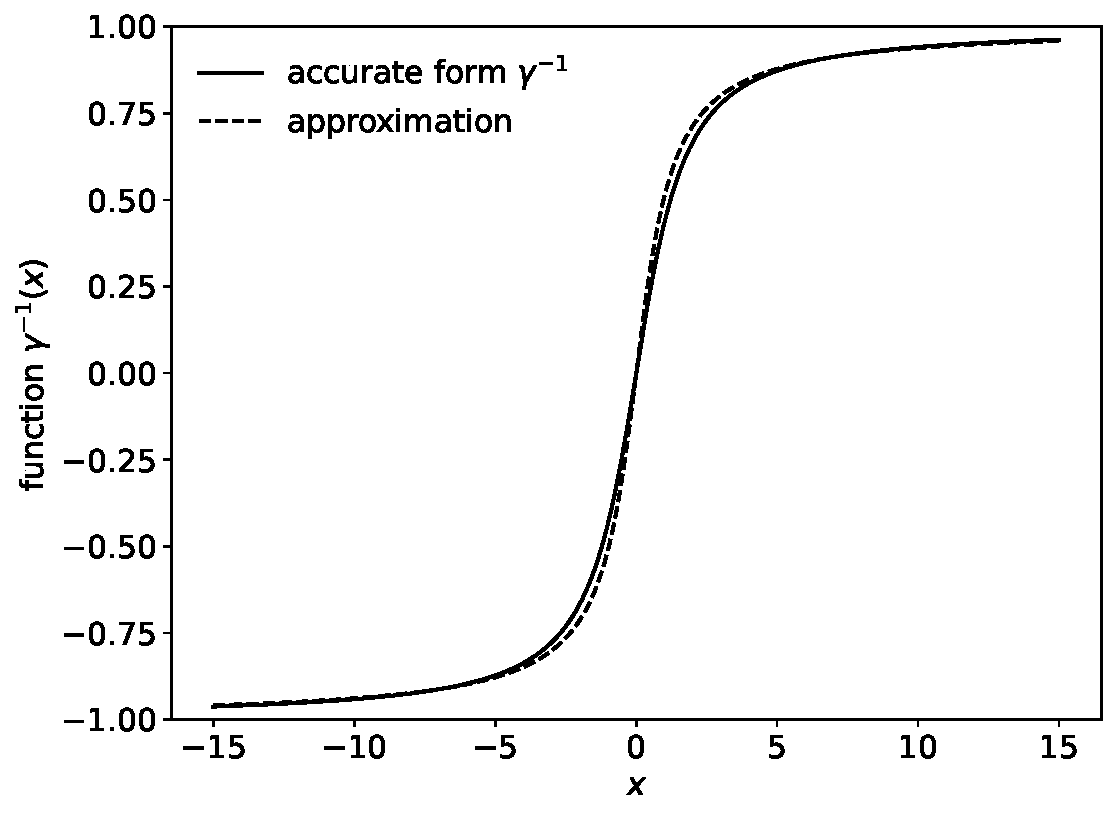
\includegraphics[width=\linewidth]{approx_invgamma.pdf}
        \caption{Auxiliary Function $\gamma^{-1}(x)$}
    \end{subfigure}
    \hfill
    \begin{subfigure}{0.48\textwidth}
        \centering
        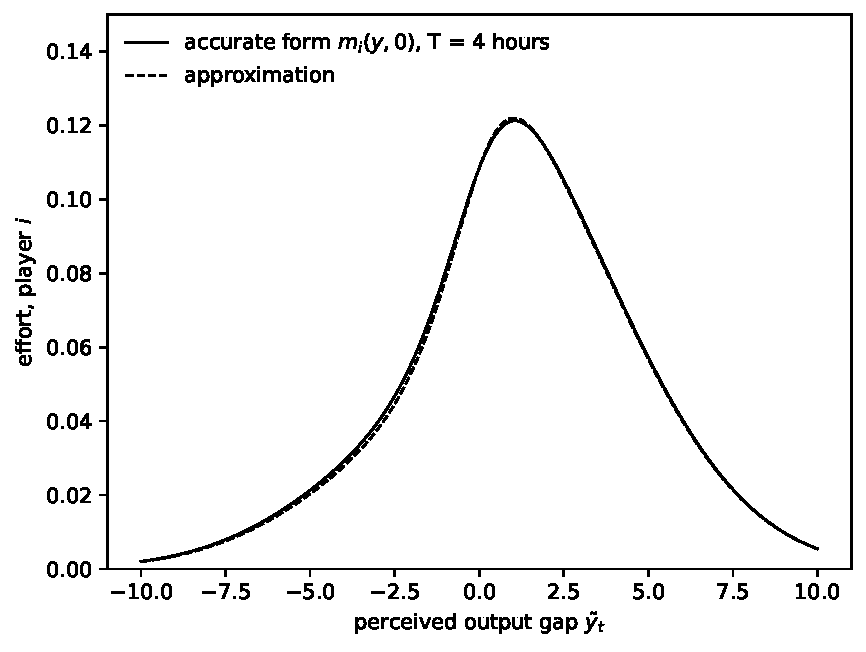
\includegraphics[width=\linewidth]{approx_equi_effort.pdf}
        \caption{Equilibrium Effort $m_i(\tilde{y}_t, t)$}
    \end{subfigure}
    \caption{Comparison of the Accurate and Approximate Forms ($\theta = 1$, $c_i = c_j = 1$, $\sigma=1$, $\Delta=1/24$)}
    \label{fig-approximation}
\end{figure}


Unknown parameters to be estimated: 
\begin{itemize}
	\item $\sigma$ (Total innovation risk): prior - truncated normal
	\item $c_i$ and $c_j$ (Capacities): prior - truncated normal
\end{itemize}



\section{Synthetic Data}

Before applying our estimation procedure to real-world contest data, we evaluate its potential on synthetically generated data.

\subsection{Data Generation}



A central challenge in generating synthetic data lies in dynamically constructing a point process that conforms to an inhomogeneous Poisson process.
We first generate candidate submission events according to a homogeneous Poisson process over the whole contest duration, using a fixed high intensity $\tau^\star \ge \sup_t \tau_{i(j)}(t)$.
Then, we apply the classical thinning procedure \citep{lewis1979simulation} to determine whether each candidate event is accepted.

\begin{algorithm}
\caption{Synthetic Data Simulation}
\begin{algorithmic}
\STATE \textbf{Input:} 
	$\Delta$, $T$, $c_i$, $c_j$, $\sigma$, $\lambda$, $r$, $\tau^\star$, $y_0$, $\mu_0$
\STATE Sample $\{s_k^{i(j)}\}^{N_{i(j)}}_{k=1}$ from homogeneous Poisson process $(\tau^\star_{i(j)})$ on $[0, T)$
\STATE Sample $\{u_k^{i(j)}\}^{N_{i(j)}}_{k=1}$ from uniform distribution on $[0, 1]$
\STATE Sample series of Brownian motions $(W_t)$ and $(B_t)$
\STATE Initialize $\ell^{i(j)}=0$, $\hat{y}_0 = 0$, $\tilde{y}_t=\mu_0$
\FOR{$t = 0$ to $T$}
    \STATE $m_{i(j)}(\tilde{y}_t, t)$  $\gets$ (\ref{eq-equilibrium-effort}), $\tau^{i(j)}(t)$ $\gets$ (\ref{eq-model-intensity})
    \hfill \COMMENT{Use $\theta$, $c_{i(j)}$, $\sigma$, $r$, $T$}
    \STATE $y_{t+\Delta} \gets$ (\ref{eq-state-dynamics}); $\tilde{y}_{t+\Delta}$ $\gets$ (\ref{eq-fintered-y-update})
    \hfill \COMMENT{Use $\sigma$, $\lambda$, $\Delta$, $W_{t+\Delta}$}
    \FOR{$s_{k}^{i(j)} \in [t, t+\Delta)$} 
        \IF {$u_k^{i(j)} < \tau_{i(j)}(s_{k}^{i(j)}) / \tau^\star_{i(j)}$}
        	    \STATE $\hat{t}^{i(j)}_{\ell} \gets s_{k}^{i(j)}$; $\ell^{i(j)} \gets \ell^{i(j)}+1$
	    \hfill \COMMENT{Accept the submission event}
	    \STATE $\hat{y}_{t+\Delta} \gets $ (\ref{eq-leaderboard-gap})
	    \hfill \COMMENT{Use $\sigma$, $\lambda$, $B_{t+\Delta}$}
        \ENDIF
    \ENDFOR
\ENDFOR
\STATE Fill in all missing entries in $(\hat{y}_t)$ by propagating the last observed value.
\STATE \textbf{Output:} $(\tilde{y}_t)$, $(\hat{y}_t)$, $\{\hat{t}_k^{i(j)}\}^{N_{i(j)}}_{k=1}$, $(m_{i(j)}(\tilde{y}_t, t))$
\end{algorithmic}
\end{algorithm}

\subsection{Bayesian Inference}

Based on the following assumptions, we will next generate the submission data for two players in a data analysis competition: 
\begin{itemize}
	\item Total uncertainty: $\sigma = 5$
	\item Capacities: $c_i = 1.5$ and $c_j = 2$
	\item Contest duration: from 2025-01-01 to 2025-03-31
	\item Starting point $\tilde{y}_0=0$
\end{itemize}

\subsection{Discussions}

...

\section{Case Study}\label{sec-kaggle-application}

...

To Do:

regression: $\lambda$ and the proportion of data release


\newpage
\section{Conclusion}


% Appendix here
% Options are (1) APPENDIX (with or without general title) or
%             (2) APPENDICES (if it has more than one unrelated sections)
% Outcomment the appropriate case if necessary
%
% \begin{APPENDIX}{<Title of the Appendix>}
% \end{APPENDIX}
%
%   or
%
% \begin{APPENDICES}
% \section{<Title of Section A>}
% \section{<Title of Section B>}
% etc
% \end{APPENDICES}

\newpage
\begin{APPENDICES}





\section{Solve $S_t$ in Equation (\ref{filtered-S})}\label{app-S-equ}

If $S$ is in steady state $dS/dt = 0$ $\Leftrightarrow$ $S = \bar{S} \equiv \sigma/\sqrt{\lambda}$. 
If $S$ is not in steady state, i.e. $S\not=\bar{S}$, we first isolate the two variables and get 
\begin{equation*}
	\frac{dS}{\sigma-\lambda S^2} = dt
\end{equation*}
Then, we take the integral on both sides
\begin{equation*}
    t = \int \frac{dS}{\sigma-\lambda S^2} = \frac{1}{\sigma\sqrt{\lambda}} \int \frac{dS\sqrt{\lambda}/\sigma}{1 - (S\sqrt{\lambda}/\sigma)^2} \equiv \frac{1}{\sigma\sqrt{\lambda}}\int \frac{du}{1-u^2} 
\end{equation*}
where $u = S\sqrt{\lambda}/\sigma = S/\bar{S}$. Hence, 
\begin{equation*}
    \sigma\sqrt{\lambda}\cdot t = \begin{cases}
        \tanh^{-1}(u)-K_1, & \text{if } |u|<1\\
        \coth^{-1}(u)-K_2, & \text{if } |u|>1
    \end{cases} = \begin{cases}
        \tanh^{-1}(S/\bar{S})-K_1, & \text{if } S<\bar{S}\\
        \coth^{-1}(S/\bar{S})-K_2, & \text{if } S>\bar{S} 
\end{cases}
\end{equation*}
Thus, we conclude the non-steady state case that 
\begin{equation*}
	S = \begin{cases}
		\bar{S}\cdot\tanh(\sigma\sqrt{\lambda}\cdot t + K_1), & \text{if } S<\bar{S}\\
		\bar{S}\cdot\coth(\sigma\sqrt{\lambda}\cdot t + K_2), & \text{if } S>\bar{S} 
	\end{cases}
\end{equation*}
Finally, we determine the constants $K_1$, $K_2$ by the initial condition $S_0$ and have 
\begin{align*}
	K_1 &= \tanh^{-1}(S_0/\bar{S})\\
	K_2 &= \coth^{-1}(S_0/\bar{S})
\end{align*}










\end{APPENDICES}



% Acknowledgments here
%\ACKNOWLEDGMENT{......}


% References here (outcomment the appropriate case)

% CASE 1: BiBTeX used to constantly update the references
%   (while the paper is being written).
%\bibliographystyle{informs2014} % outcomment this and next line in Case 1
%\bibliography{<your bib file(s)>} % if more than one, comma separated

% CASE 2: BiBTeX used to generate mypaper.bbl (to be further fine tuned)
%\input{mypaper.bbl} % outcomment this line in Case 2

%If you don't use BiBTex, you can manually itemize references as shown below.


%\bibliographystyle{nonumber}
\bibliographystyle{informs2014}
\bibliography{_Literatures.bib}

%%%%%%%%%%%%%%%%%
\end{document}
%%%%%%%%%%%%%%%%%
